\documentclass{standalone}
\usepackage{tikz}
\usepackage{amssymb}
\usetikzlibrary{automata, positioning}

\begin{document}
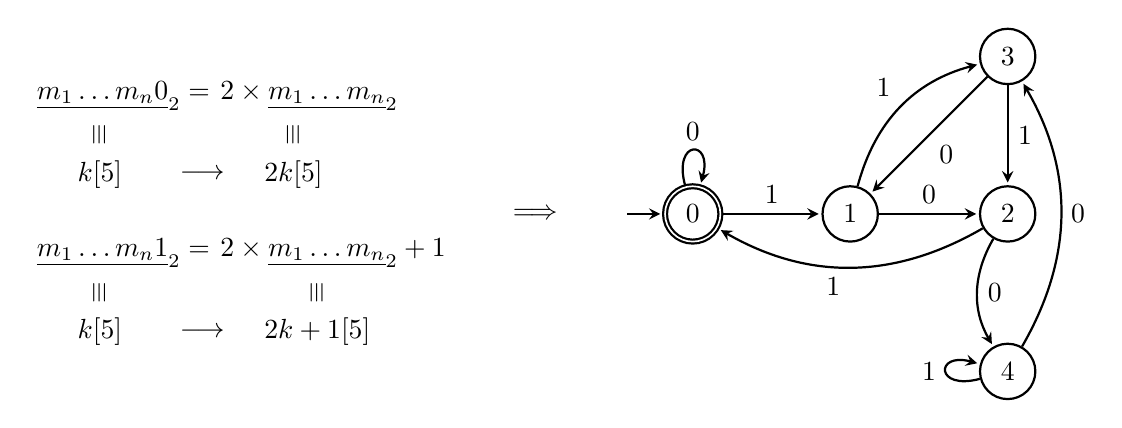
\begin{tikzpicture}[%
    >=stealth,
    shorten >=1pt,
    node distance=2cm,
    on grid,
    auto,
    state/.append style={minimum size=2em},
    thick
  ]
  \node[anchor=east] at (-4,1.5) (E1_1) {$\underline{m_1\dots m_n0}_2 = $};
  \node[right = 1.1 of E1_1, anchor=west] (E1_2) {$2 \times \underline{m_1 \dots m_n}_2$};
  \node[below left = 0.5 and 0.3 of E1_1, rotate=90 ] (equiv1_1) {$\equiv$} ;
  \node[below left = 0.5 and 0.2 of E1_2, rotate=90 ] (equiv1_2) {$\equiv$} ;
  \node[below = 0.5 of equiv1_1] (k_1) {$k[5]$} ;
  \node[below = 0.5 of equiv1_2] {$2k[5]$} ;
  \node[right= 1.3 of k_1] {$\longrightarrow$};

  \node[anchor=east] at (-4,-.5) (E2_1) {$\underline{m_1\dots m_n1}_2 = $};
  \node[right = 1.1 of E2_1, anchor=west] (E2_2) {$2 \times \underline{m_1 \dots m_n}_2 + 1$};
  \node[below left = 0.5 and 0.3 of E2_1, rotate=90 ] (equiv2_1) {$\equiv$} ;
  \node[below left = 0.5 and 0.2 of E2_2, rotate=90 ] (equiv2_2) {$\equiv$} ;
  \node[below = 0.5 of equiv2_1] (k_2) {$k[5]$} ;
  \node[below = 0.5 of equiv2_2] {$2k + 1[5]$} ;
  \node[right= 1.3 of k_2] {$\longrightarrow$};
 
  \node[] at (0, 0) (implies) {$\Longrightarrow$};

  \node[state, initial, initial text = {}, accepting, right = of implies] (0) {$0$};
  \node[state] (1) [right= of 0] {$1$};
  \node[state] (2) [right= of 1] {$2$};
  \node[state] (3) [above= of 2] {$3$};
  \node[state] (4) [below= of 2] {$4$};
  \path[->] 
            (0) edge [loop above] node {0} (0)
            (0) edge [] node {1} (1)
            (1) edge [] node {0} (2)
            (1) edge [bend left] node {1} (3)
            (2) edge [bend right] node {0} (4)
            (2) edge [bend left] node[below left] {1} (0)
            (3) edge [] node {0} (1)
            (3) edge [] node {1} (2)
            (4) edge [bend right] node[right] {0} (3)
            (4) edge [loop left] node {1} (4);
\end{tikzpicture} 
\end{document}